\section{{Resultados}}

La tabla \ref{{tab:clean-up-results}} muestra las cantidades de ensayos
obtenidos y su considerable reducción luego de aplicar los criterios de
filtrado.

tabla \ref{{tab:correcteness-rates}}

tabla \ref{{tab:response-times}}

figura \ref{{fig:first-starting-sample-distribution}}

figura \ref{{fig:second-starting-sample-distribution}}

TODO: Hacer \verb|\ref| a las tablas y figuras que describen un poco todo

TODO: Sacadas correctivas

De las respuestas incorrectas, {first__corrected_sample__trials_count} tuvieron
una segunda sacada correctiva antes del fin del ensayo, es decir que tras mirar
al punto incorrecto, corrigió y realizó una sacada hacia el punto correcto.

En un {second__antisaccades_correction_percentage}$\%$ de las antisacadas
incorrectos se realizó una corrección.
Tal corrección tomó en promedio
{second__corrected_antisaccades_sample__mean_correction_delay} ms (stdev
{second__corrected_antisaccades_sample__stdev_correction_delay} ms).

\begin{{table}}
  \centering
  \begin{{tabular}}{{ c c | c | c }}
    \multicolumn{{2}}{{c|}}{{ronda}} & primera & segunda \\ 
    \hline
    \multirow{{2}}{{10em}}{{pre-limpieza}}
      & sujetos
      & {first__starting_sample__subjects_count}
      & {second__starting_sample__subjects_count} \\  
      & ensayos
      & {first__starting_sample__trials_count}
      & {second__starting_sample__trials_count} \\  
    \hline
    \multirow{{2}}{{10em}}{{post-limpieza}}
      & sujetos
      & {first__inlier_sample__subjects_count}
      & {second__inlier_sample__subjects_count} \\  
      & ensayos
      & {first__inlier_sample__trials_count}
      & {second__inlier_sample__trials_count} \\  
    \hline
    \multirow{{2}}{{10em}}{{proporción conservada}}
      & sujetos
      & {first__kept_subjects_percentage}\%
      & {second__kept_subjects_percentage}\% \\  
      & ensayos
      & {first__kept_trials_percentage}\%
      & {second__kept_trials_percentage}\% \\  
  \end{{tabular}}

  \caption{{Ensayos pre y post limpieza}}
  \label{{tab:clean-up-results}}
\end{{table}}

\begin{{table}}
  \centering
  \begin{{tabular}}{{c | c | c c}}
    ronda
      & primera
      & \multicolumn{{2}}{{c}}{{segunda}} \\
    tarea
      & antisacada
      & antisacada
      & prosacada \\
    \hline
    tasa de correctitud
      & {first__antisaccades_correctness_percentage}\%
      & {second__antisaccades_correctness_percentage}\%
      & {second__prosaccades_correctness_percentage}\% \\
  \end{{tabular}}
  \caption{{Tasas de correctitud}}
  \label{{tab:correcteness-rates}}
\end{{table}}

\begin{{table}}
  \centering
  \begin{{tabular}}{{c|cc|cccc}}
    ronda
      & \multicolumn{{2}}{{|c|}}{{primera}}
      & \multicolumn{{4}}{{|c|}}{{segunda}} \\
    tarea
      & \multicolumn{{2}}{{|c|}}{{antisacada}}
      & \multicolumn{{2}}{{|c }}{{antisacada}}
      & \multicolumn{{2}}{{ c}}{{prosacada}} \\
    correctitud
     & correcto & incorrecto
     & correcto & incorrecto
     & correcto & incorrecto \\
    \hline
    tiempo de respuesta en
     &  {first__correct_antisaccades_sample__mean_response_time}
       ({first__correct_antisaccades_sample__stdev_response_time})
     &  {first__incorrect_antisaccades_sample__mean_response_time}
       ({first__incorrect_antisaccades_sample__stdev_response_time})
     &  {second__correct_antisaccades_sample__mean_response_time}
       ({second__correct_antisaccades_sample__stdev_response_time})
     &  {second__incorrect_antisaccades_sample__mean_response_time}
       ({second__incorrect_antisaccades_sample__stdev_response_time})
     &  {second__correct_prosaccades_sample__mean_response_time}
       ({second__correct_prosaccades_sample__stdev_response_time})
     &  {second__incorrect_prosaccades_sample__mean_response_time}
       ({second__incorrect_prosaccades_sample__stdev_response_time}) \\
    ms, promedio (desvio std) & & & & & & \\
  \end{{tabular}}
  \caption{{Tiempos de respuesta}}
  \label{{tab:response-times}}
\end{{table}}

\begin{{figure}}
  \centering

  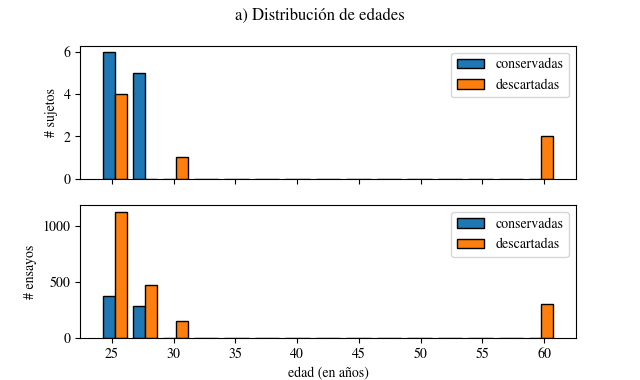
\includegraphics[width=0.8\linewidth]{{results/first-ages-distribution.png}}

  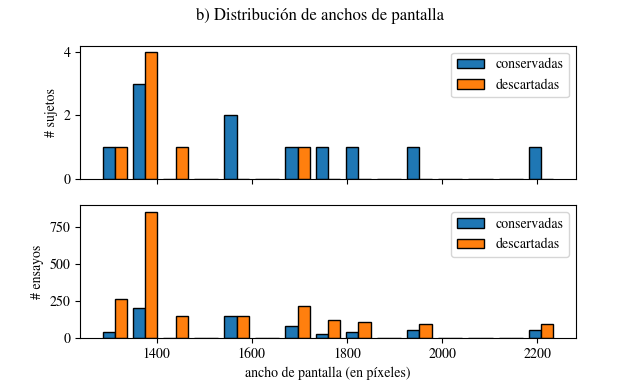
\includegraphics[width=0.8\linewidth]{{results/first-widths-distribution.png}}

  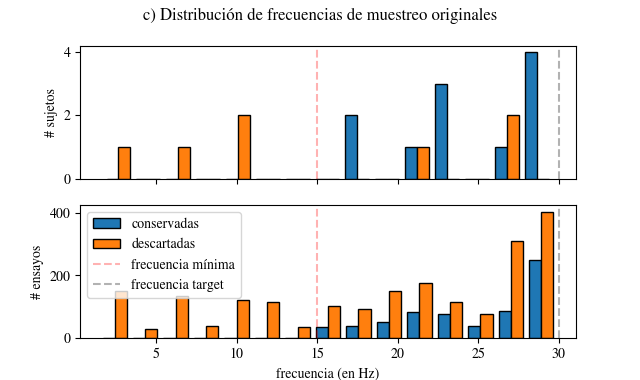
\includegraphics[width=0.8\linewidth]{{results/first-sampling-frequencies-distribution.png}}

  \caption{{Descripción general (primera instancia)}}
  \label{{fig:first-starting-sample-distribution}}
\end{{figure}}

\begin{{figure}}
  \centering

  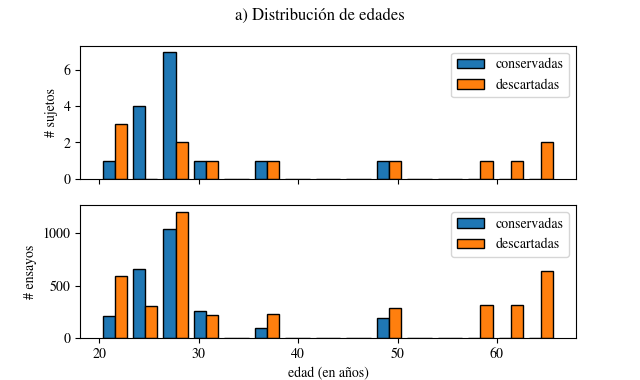
\includegraphics[width=0.8\linewidth]{{results/second-ages-distribution.png}}

  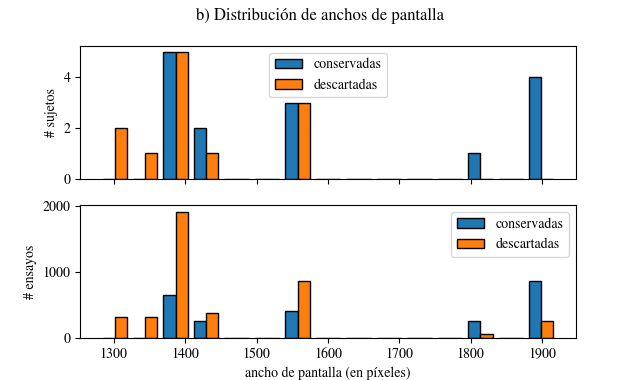
\includegraphics[width=0.8\linewidth]{{results/second-widths-distribution.png}}

  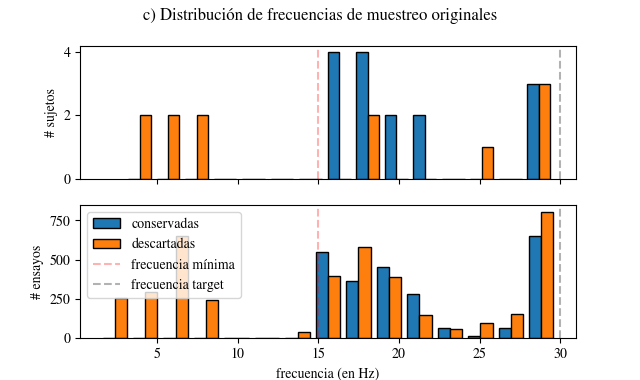
\includegraphics[width=0.8\linewidth]{{results/second-sampling-frequencies-distribution.png}}

  \caption{{Descripción general (segunda instancia)}}
  \label{{fig:second-starting-sample-distribution}}
\end{{figure}}

TODO: Las tres figuras con ensayos desagregados por correctitud

TODO: Las dos figuras con las distribuciones de los tiempos de respuesta


TODO: Algún comentario más concreto sobre las desviaciones?

TODO: Alguna figura sobre las desviaciones?


Pudieron replicarse resultados generales esperados en la tarea de antisacadas.
Las antisacadas incorrectas mostraron tiempos de respuesta menores que las
antisacadas correctas.
Esto es consistente con la noción de que realizar correctamente la tarea
implica un costo cognitivo adicional.
En la primera instancia de experimentación se obtuvo, para la tarea de
antisacadas, una tasa de correctitud dentro del rango esperable.
Mientras que en la segunda fue mayor, pero sí se comportó como era esperado ya
que fue mayor para el caso prosacada que para antisacada.

TODO: Nula representatividad de gente mayor

TODO: Figura de frecuencia de muestreo en función de la edad


TODO: Baja representatividad de grupo incorrecto por sujeto

TODO: Tabla cantidades de correctitud por sujeto de la segunda instancia

{second__correctness_summary_table}

%

TODO: Rever la conclu para que no se repita con esta sección

%%%%%

\subsection{{Primera instancia}}

\begin{{figure}}
  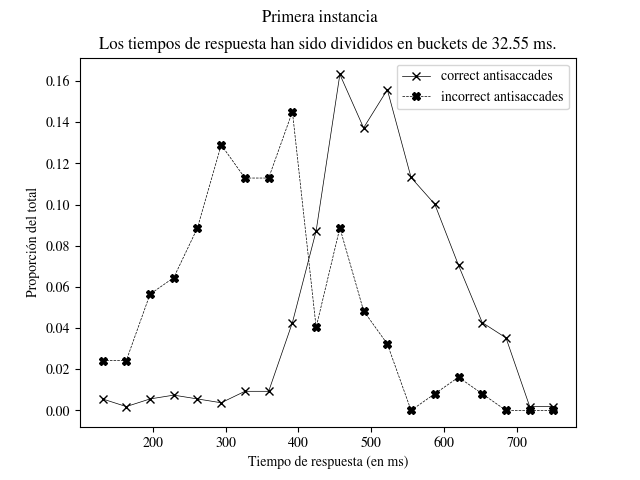
\includegraphics{{results/first-response-times-distribution.png}}
  \caption{{Distribución de tiempos de respuesta (primera instancia)}}
  \label{{fig:first-response-times-distribution}}
\end{{figure}}

\begin{{figure}}
  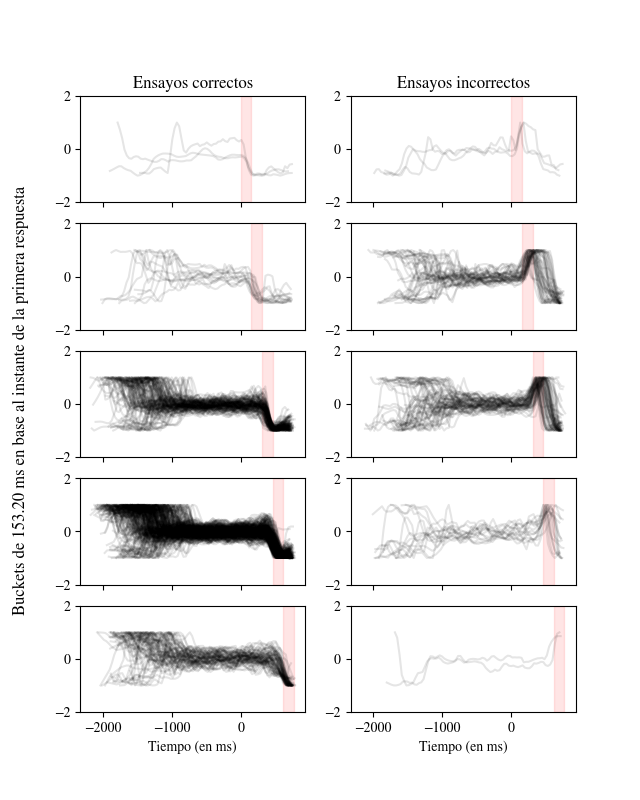
\includegraphics{{results/first-disaggregated-antisaccades.png}}
  \caption{{Antisacadas desagregadas (primera instancia)}}
  \label{{fig:first-disaggregated-prosaccades}}
\end{{figure}}

\subsubsection{{Estimaciones desviadas}} \label{{section:skewed-estimates}}

Se encontró que para varios sujetos [TODO: cuántos sujetos? con qué magnitud?]
las estimaciones obtenidas estaban desviadas del centro (Figura
\ref{{fig:skewed-estimations-example}}).
Para cada sujeto, estas desviaciones fueron consistentes a lo largo de todo el
experimento.
Además se mantuvo la posición relativa de las estimaciones.
Luego de ser apropiadamente normalizados, se logró entonces utilizar los datos
recolectados para identificar si la mirada caía en algunas de las tres regiones
de interés.

\begin{{figure}}
  \centering

  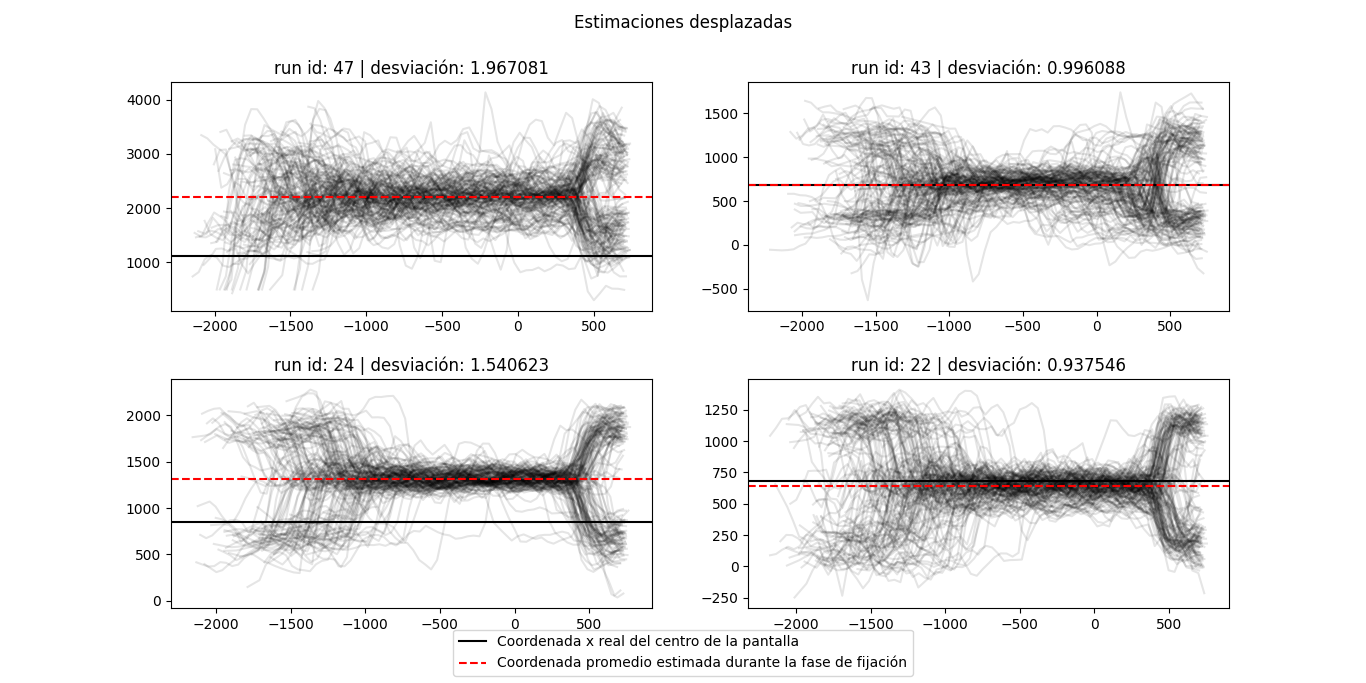
\includegraphics[width=\textwidth]{{results/skewed-estimations.png}}
  Durante la fase de fijación los sujetos 47 y 24 obtuvieron respectivamente
  estimaciones cercanas a los 2100 y 1400 píxeles, cuando los valores reales
  serían 1100 y 900.
  Estas desviaciones no ocurrieron para todo sujeto, como lo muestran los
  sujetos 42 y 22. \\
  El valor de desviación reportado se calcula como la división entre la
  coordenada estimada del centro (el promedio de las estimaciones durante el
  período de fijación) y la coordenada real del centro.

  TODO: Regenerar este plot para que macheen las dimensiones

  \caption{{Ejemplos de sujetos con estimaciones desviadas}}
  \label{{fig:skewed-estimations-example}}
\end{{figure}}

\subsection{{Segunda instancia}}

\begin{{figure}}
  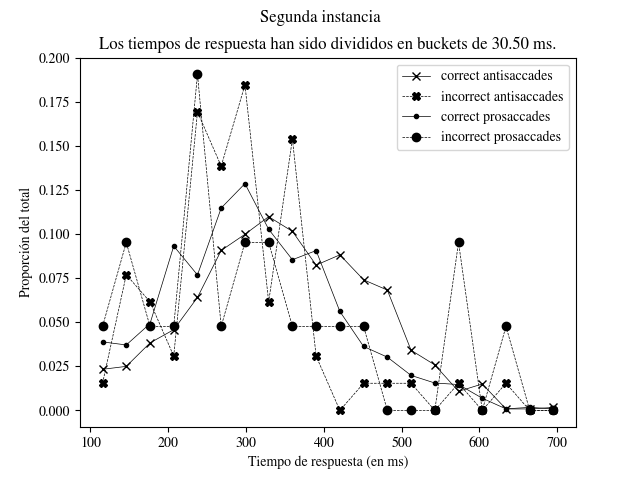
\includegraphics{{results/second-response-times-distribution.png}}
  \caption{{Distribución de tiempos de respuesta (segunda instancia)}}
  \label{{fig:second-response-times-distribution}}
\end{{figure}}

\begin{{figure}}
  \centering
  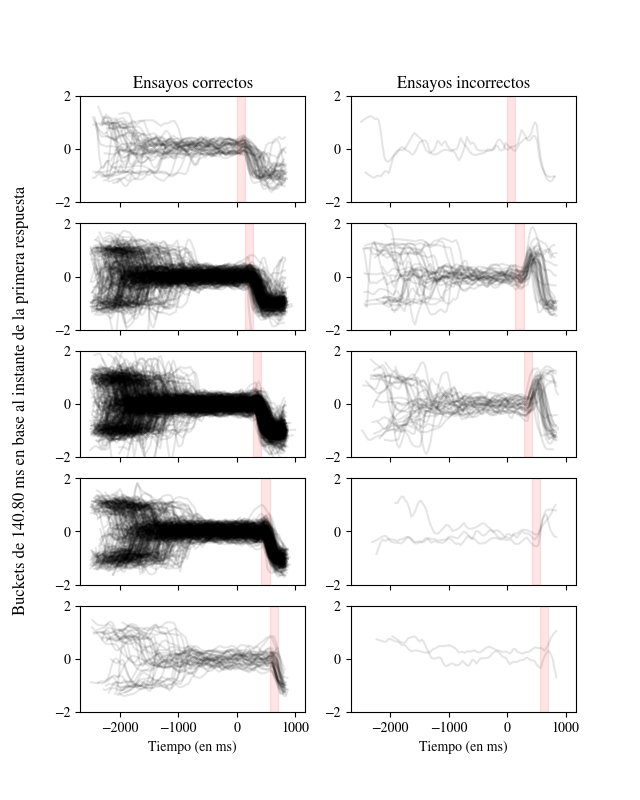
\includegraphics{{results/second-disaggregated-antisaccades.png}}
  \caption{{Antisacadas desagregadas (segunda instancia)}}
  [TODO: \\
  - Acá estaba explicando comentando que los datos estaban normalizados pero la
  verdad que no aporta.
  Sí comentar sobre los datos alineados temporalmente el efecto de la
  normalización en la \textit{{apariencia}} final de los datos.
  Lo mismo para la figura de prosacadas y para la de la primera instancia.
  Capaz se las pueda unificar y hacer en simultáneo comentario de las tres.]
  \label{{fig:second-disaggregated-antisaccades}}
\end{{figure}}

\begin{{figure}}
  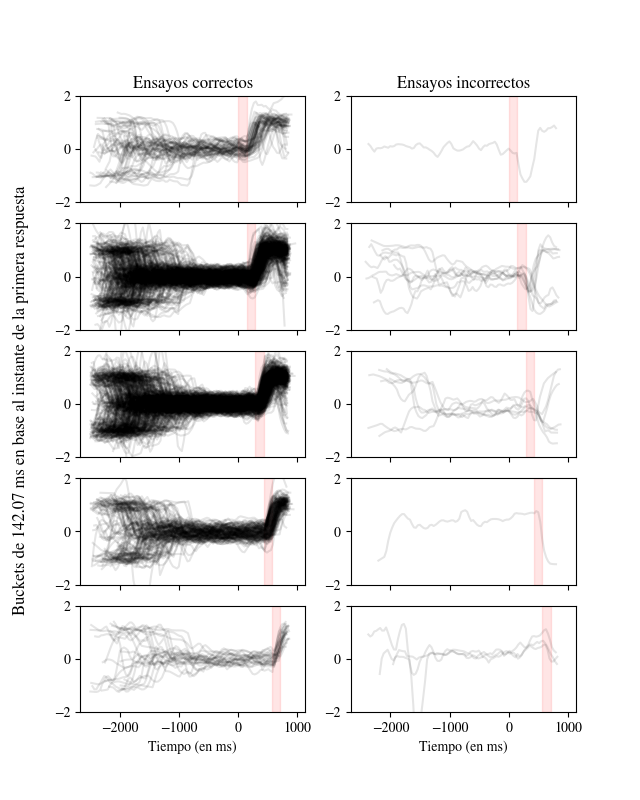
\includegraphics{{results/second-disaggregated-prosaccades.png}}
  \caption{{Prosacadas desagregadas (segunda instancia)}}
  \label{{fig:second-disaggregated-prosaccades}}
\end{{figure}}

\begin{{figure}}
  \centering
  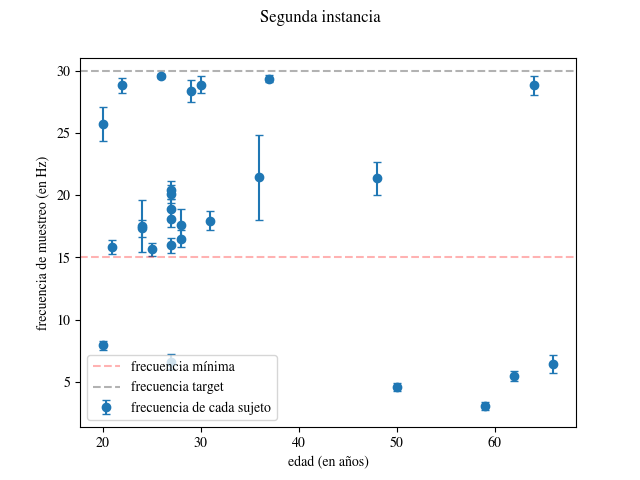
\includegraphics[width=\textwidth]{{
    results/second-sampling-frequencies-by-age.png}}
  \caption{{Frecuencia de muestreo en función de la edad}}
  [TODO: \\
  - Regenerar plot y ajustar dimensiones \\
  - Debería escribir algún comentario acá?]
  \label{{fig:sampling-frequencies-by-age}}
\end{{figure}}
